%===================================== CHAPTER 8 Implementation =================================

\chapter{Implementation}

This chapter discusses the details of the system implementation process, both for front end and for back end.


\section{Project Progression}
Project progression is derived from the activity \ref{app:activityplan}, meeting abstracts\ref{app:meetingabstract) and Trello archive \todo {Blir dette referet til? + legg inn ref her. Står det noe om hvor lange sprintene er tidliger? når de slutter of started klokkeslett}  and will only briefly summarize what was done at each sprint.

\begin{description}
	
	\item[Sprint 1 - 23.01.15 - 30.01.15] \hfill \\ 
	The first week mainly consisted of getting familiar with each other and the assignment. as soon as the introductions was done we talked about our personal goals to set the expectation as a group and we formalized a Rule of engagement\ref{app:rulesofengagement} for the group to sign, also dispersed responsibilities. Later we established a meeting agenda with the customer and met for the first time.
	
	\item[Sprint 2 - 30.01.15 - 06.02.15] \hfill \\ 
	Sprint 2 we begun planning and formalizing the requirements after. large section of work like sketching a WBS \ref{wbs}, generating a product backlog \ref{productbacklog}, and Use Cases was done this week. Other design work like the architecture and UI mockups where started on.
	
	\item[Sprint 3 - 06.02.15 - 13.02.15] \hfill \\ 
	This was the first week of development. We started testing the API \ref{subsec:api} and finalized some paper prototypes for testing \todo{Referanse til papirprototype} and also completed database and architecture design. Research towards the personalization, the front end framework \ref{subsec:ionic} \todo{ref:personalization} and differences between the two operation systems \todo{ref crossplatform OS}. 
	
	\item[Sprint 4 - 13.02.15 - 20.02.15] \hfill \\ 
	Analyzing the past work \ref{subsec:stedr} to see if would fit out needs, continuing the research towards collaborative filtering \ref{sec:personalization_algorithms}. and learning docker \ref{subsec:docker}. labor as mapping the Digitalt fortalt \todo{ref} categories to our own and conducting and evaluating the paper prototype test as well as the database code was taking shape.
	
	\item[Sprint 5 - 20.02.15 - 27.02.15] \hfill \\ 
	
		
	\item[Sprint 6 - 27.02.15 - 06.03.15] \hfill \\ 

	\item[Sprint 7 - 06.03.15 - 13.03.15] \hfill \\ 
	
	\item[Sprint 8 - 13.03.15 - 20.03.15] \hfill \\ 

	\item[Sprint 9 - 20.03.15 - 27.03.15] \hfill \\ 
	
	\item[Easter - 27.03.15 - 07.04.15] \hfill \\ 
	The application was tested under informal condition on family and friends. "in the wild" test
	\item[Sprint 10 - 08.04.15 - 17.04.15] \hfill \\ 

	\item[Sprint 11 - 17.04.15 - 24.04.15] \hfill \\ 

	\item[Sprint 12 - 24.04.15 - 01.05.15] \hfill \\ 
	
	\item[Sprint 13 - 01.05.15 - 08.05.15] \hfill \\ 

	\item[Sprint 14 - 08.05.15 - 15.05.15] \hfill \\ 
	
	\item[Past 15.05.15] \hfill \\ 
	Work was conducted after the last sprint(sprint 14) this was was fixing crucial bugs on the applikation the finalizing the report as well as carry out an acceptance test \todo{ref acceptance test} with the custumer
	
\end{description}


\section{Front end}

The front end of the application was designed by using Ionic and AngularJS. In this section, there will first be a description of how a system made in AngularJS is structured, and in the subsequent section will be an elaboration of some challenges and limitations during the creation of the user interface, both concerning the design and the implementation aspects of the process.

\subsection{AngularJS system structure}

AngularJS is based on a Model-View-Controller architecture, but provides a variety of components to assist in easing the programming and speeding up the application. It is essentially another layer of abstraction above writing regular Javascript. These are some of the main concepts that are used to create an Angular application:

\begin{description}
	\item[Model] \hfill \\ 
	The data that can be interacted with by the user.
	
	\item[View] \hfill \\ 
	The interfaces that the user can see.
	
	\item[Controller] \hfill \\ 
	The logic and behavior of the views.
	
	\item[Directive] \hfill \\ 
	Special functionality applied to the DOM elements, you can create your own directives as well as use the numerous ones provided by AngularJS itself. In "Vettu hva?", several of these were used, such as directives that call on some function when DOM elements are clicked on, or directives that show or hide parts of the DOM based on some condition.
	
	\item[Module] \hfill \\ 
	A module encapsulates a part of the application. Instead of having a single "main" function that holds the application together, Angular applications normally have multiple modules that work together. The benefit of this is that the application is decomposed into logical parts that can be reused, loaded, and tested in any order. In "Vettu hva?", each controller is its own module. The part of the program that communicated with the back end is also encapsulated in a module. Furthermore, there is a module that starts up the application and binds together views and controller into different states.
	
	\item[Scope] \hfill \\ 
	The scope contains all the elements that the application currently has access too. It can be viewed as a container that stores the current model, and so if a controller or directive is going to modify or access the model, this has to be done by using the scope.
	
	\item[Service] \hfill \\ 
	A service contains "global" logic that is accessible to the entire application. In "Vettu hva?", this is used in the module that contains the communication with the back end. This module has three different services, which respectively gives the application access to User data, story data, and requests from front end to back end.
\end{description}

\subsection{User interface}

Early on in development, the team discovered several limitations of the Ionic framework. For example when using a list to display stories, it was not possible to swipe the list both left and right. The idea was to swipe one way to add a story to be read later, and swipe the other way to reject a story from the list entirely.  Because this proved to be impossible, the views were redesigned into a different solution which was much less based around swiping.\newline

As this is an application for mobile devices, it had to be adapted to work on different screen sizes. The team found that it would most likely be best to target a relatively small screen size and then simply enlarge it for bigger screens. This eliminated the issue of having to compress the components to fit smaller screen sizes and potentially be forced to redesign the whole view to fit small screens.\newline

The applications uses many different icons in various parts of the interface, and these have been the source of much debate and redesign. The icons used to represent categories were not always understood by users, and some categories like “local tradition and food” were difficult to represent universally with just a single icon. Also the bookmark icon shown in the upper right area of figure 8.xx was confusing to many users, and there was a concern in the team that this icon might not accurately represent that it allows the user to save the story in a collection.\newline

Adopting accurate naming conventions for the different components has also been a considerable issue. Stories can be saved in collections, but these collections have interchangeably been called lists, tags, and bookmarks in the system. Also when asking a user to input their preferred categories to receive stories from, there has been some confusion because of interchangeably calling these categories for interests,  preferences, and categories.\newline

Implementing media, and especially video, has been a challenge in the project. An issue with this has been that playing videos is handled differently on iOS and Android, which had resulted in some bugs that only appear on one platform and not the other. These types of issues have been problematic to fix and has taken up much time to fix. In addition, the videos provided by the Digitalt fortalt website come from different sources. Some of them are Youtube videos, others are Vimeo videos, and there are also other variations. Integrating all these different formats smoothly into the application has been a challenge in itself.

\subsection{Prototype}

The prototype has been through multiple iterations. Early on, it was imagined to have a sort of “magic” discovery function where a user would for example rub a crystal ball and receive a recommended story. This idea was later discarded because the team decided it would be better usability to present the user with multiple recommended story that they could simply browse through instead.\newline

Another of the early ideas was for the user to receive a “daily story” or some sort of schedule for being presented with recommended stories. However, due to workload and time constraints, this requirement was heavily down prioritized. The most important parts were the personalization and usability aspects, so receiving notifications seemed like an unnecessary extra feature.\newline

A big issue for the interface design has been the handling of the different media elements (text, pictures, audio, video) and how these should be positioned relative to each other. For a while the team designed the application to have one tab for each of these four elements in the story view, as shown to the left in figure 8.XX. The customer had a concern that this might not be the optimal solution, as a user would for example not be able to read text and view pictures simultaneously. After some discussion, the interface was redesigned so that the text would be persistent, and instead the user could tab between pictures, audio, and video. The resulting design can be seen to the right in \textbf{Fig \ref{Fig:prototype}}. 

\begin{figure}
	\centering
	\begin{subfigure}[h]{0.4\textwidth}
		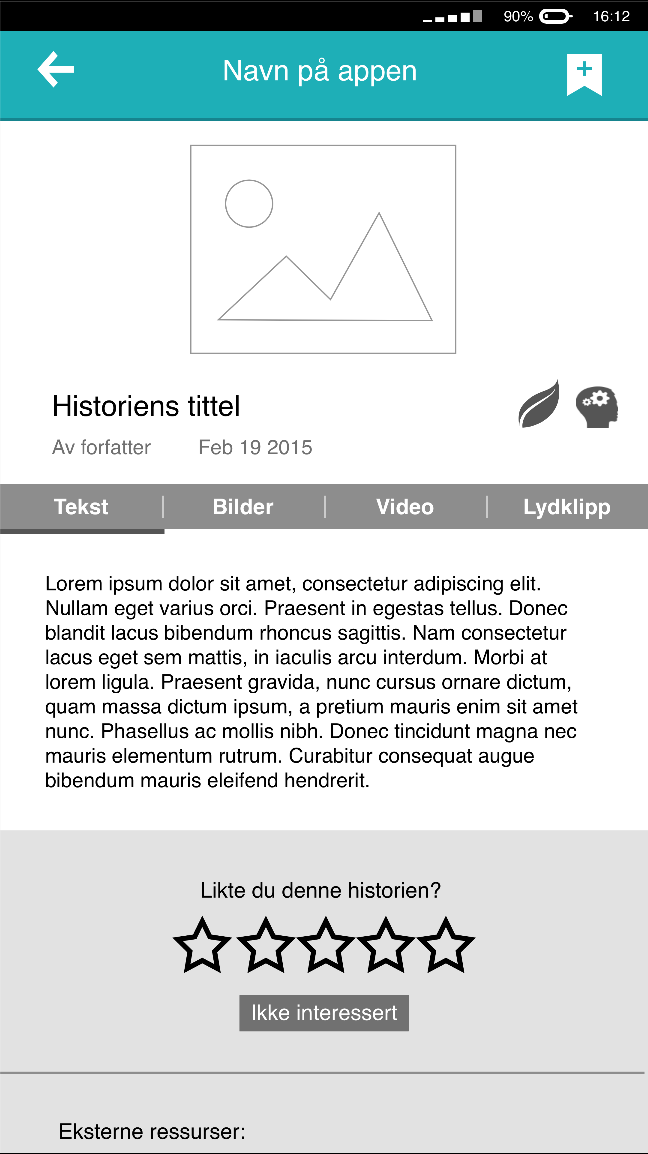
\includegraphics[width=\textwidth]{fig/prototype1}
	\end{subfigure}
	%
	\begin{subfigure}[h]{0.4\textwidth}
		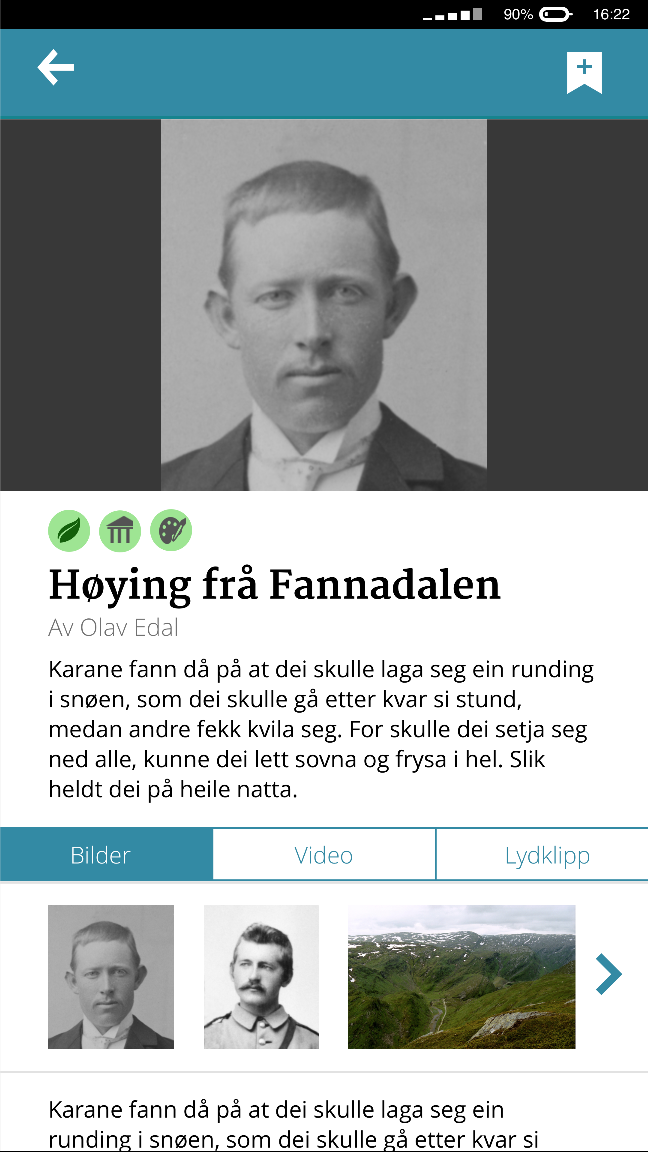
\includegraphics[width=\textwidth]{fig/prototype2}
	\end{subfigure}
	\caption{Comparison of the story view in the first and second version of the prototype.}
	\label{Fig:prototype}
\end{figure}

\section{Back end}

This section describe the development of each part of the back end. It aims to give a timeline of the development and explain how and why important decisions were made. The different parts described here are the database and the personalization. 

\subsection{Database}

Based on the first version of the functional requirements for the application an initial ER-diagram was made in the middle of February. At this stage the customer and the team had not come to an agreement on a prioritization of the non-functional requirements. This meant that there for instance was not clear how important the performance of the system would be for the customer, an attribute of the system which would influence how much info should be stored for each story in the database versus have much info should be retrieved from Digitalt fortalt every time a user views a story. However, the changes to the initial diagram have been relatively minor. Some of the alterations were based on updated requirements from the customer, while others stem from the group and are optimization of the data model or changes made to facilitate the personalization. \newline

Shortly after the first ER-diagram was made, an SQL script for creating a database was also made. Since the ER-diagram has undergone changes for quite some time after the first version was made, these changes has also influenced the SQL script. This means that a change in the data model have lead to more work than just updating the ER-diagram. However, the progress of the project relied on testing against an operational database, for instance regarding the harvesting of stories from Digitalt fortalt. \newline

The customer had early on said that the retrieval of research data about the use of the application was important for them. Initially, the details of this was not properly formulated and the initial data model therefore did not reflect this. After receiving a detailed list from the customer describing the research data to be gathered, alterations - mostly additions - in the data model were made to accommodate this. This concerned storing timestamps for user actions and states of stories.  \newline

The team did not decide or understand how to do the personalization until mid March. This decision introduced changes to existing tables and the need to create additional tables and views in the database. Mahout had requirements for the input data, which meant that a view was created to store all the necessary data for collaborative filtering. Using this view made it straightforward to put the desired data from the database into Mahouts data model.

\subsection{Personalization}

At the start of the project much time was devoted to understanding content-based and collaborative filtering and how the theoretical descriptions of these techniques could be turn into a practical implementation in our application. When the back end part of the group had a better understanding on how this could be done, an important decision was whether to use open source recommender engines or to implement the algorithms ourselves. After studying the math and complexity involved in writing our own implementation it became clear that the best solution would be to use existing recommender engines, even if this would require some adjustments to already written code. \newline

As the project was nearly halfway through when the decision to use an open source recommender engine was made, the team did not find the time to do a thorough review of the many different alternatives. This increased the probability of choosing the wrong tool to work with and violated the stated preventive action in the risk list (see \textbf{appendix \ref{app:risklist}}). However, the customer suggested three different recommender engines that might be worth looking into, one of which was Mahout. In choosing a tool the customer had done some research on, the group found that the risk of doing a wrong choice decreased somewhat. In addition, Mahout presented its features in a way that resembled the groups research on filtering algorithms and it was therefore reason to believe that getting started with Mahout would not require much additional research. Of particular importance was the fact that Mahout offered an explanation on how to do content-based filtering using their recommender engine. Most such engines provided functionality for doing collaborative filtering, but it was not always clear how content-based filtering could be done.\newline

Mahouts website provided some guiding on how to build a recommender which made it possible to use the tool without thorough knowledge of how the different methods worked. Most work in the beginning of doing the personalization thus centered around how to gather and produce data in a format acceptable to Mahout and how to treat the output recommendations. Content-based filtering was implemented first, as this was the customer's wish and because the first recommendations presented to a user would always be content-based. Since Mahout does not provide methods for finding similarities between items based on their attributes, the group had to implement this. There exist a vast number of functions to compute similarity between objects. The group did some research on different similarity measures, but the literature did not provide an clear-cut answer which measure was best fitted to our data. Cosine similarity was chosen for its simplicity and because a story's subcategories lent itself well to be represented as a vector.\newline

The customer requested the use of both item based and user based collaborative filtering. There was some doubt in the group as to whether the produced recommendations from the two methods could be combined, but it was found that this was possible as both take the same data model as input. When doing user based collaborative filtering, a threshold value had to be set to tell the recommender engine which users should affect the recommendations. This concerns the similarity found between users. It was difficult to set this value as the computation of the similarity is done by Mahout and because the group did not know what threshold value would be reasonable to set. The value is set by means of trial and error looking at the resulting recommendations produced using different values, and by looking at example use of this method. 


\cleardoublepage